\begin{frame}{Boosting}

\begin{itemize}
    \item Boosting refers to an ensemble method in which many predictors are trained and each predictor learns from the errors of its predecessor. \pause 

    \item  More formally, in boosting many \textbf{weak learners} are combined to form a \textbf{strong learner}. \pause

    $\rightarrow$A weak learner is a model doing slightly better than random guessing.  \pause 

    \item Here, an ensemble of predictors are trained \textit{sequentially} and each predictor tries to correct the errors made by its predecessor. \pause 
    \item Boosting has three tuning parameters:

    \begin{enumerate}
        \item \textbf{The number of trees $B$}: selected by cross-validation. \pause 

        \item \textbf{The shrinkage parameter $\eta$}: this controls the rate at which boosting learns. \pause 

        \item \textbf{The number $d$ of splits in each tree}: which controls the complexity of the boosted ensemble.
    \end{enumerate}

    
\end{itemize}
    
\end{frame}

\begin{frame}{Boosting}
\begin{figure}
    \centering
    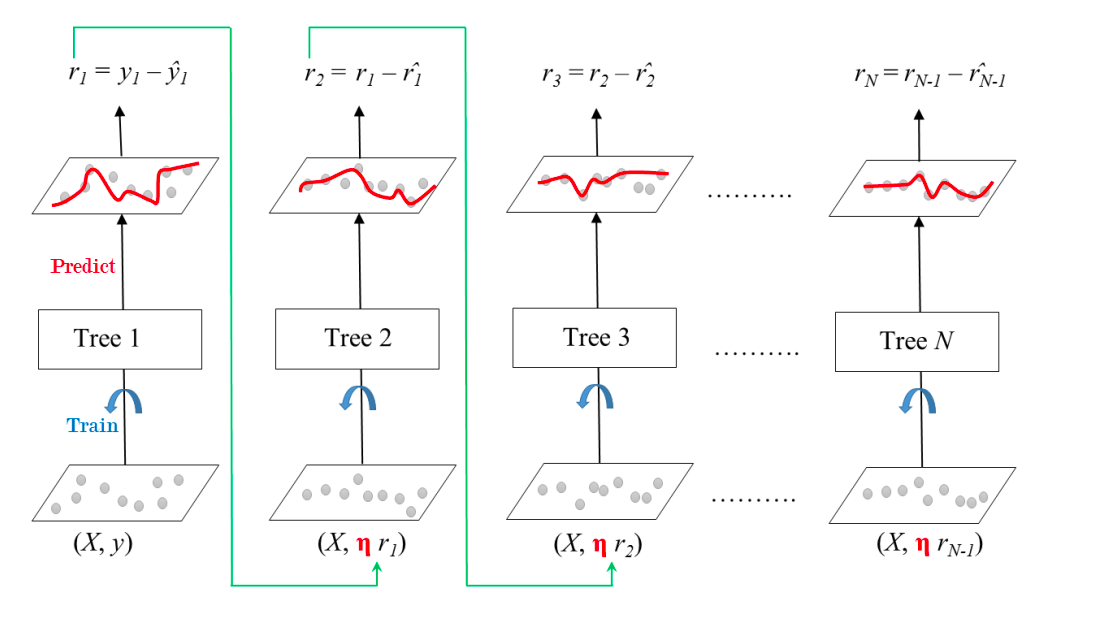
\includegraphics[height=6cm]{bagging-boosting/boosting.png}
\end{figure}
    
\end{frame}